\documentclass[11pt]{article}\usepackage[]{graphicx}\usepackage[]{color}
%% maxwidth is the original width if it is less than linewidth
%% otherwise use linewidth (to make sure the graphics do not exceed the margin)
\makeatletter
\def\maxwidth{ %
  \ifdim\Gin@nat@width>\linewidth
    \linewidth
  \else
    \Gin@nat@width
  \fi
}
\makeatother

\definecolor{fgcolor}{rgb}{0.345, 0.345, 0.345}
\newcommand{\hlnum}[1]{\textcolor[rgb]{0.686,0.059,0.569}{#1}}%
\newcommand{\hlstr}[1]{\textcolor[rgb]{0.192,0.494,0.8}{#1}}%
\newcommand{\hlcom}[1]{\textcolor[rgb]{0.678,0.584,0.686}{\textit{#1}}}%
\newcommand{\hlopt}[1]{\textcolor[rgb]{0,0,0}{#1}}%
\newcommand{\hlstd}[1]{\textcolor[rgb]{0.345,0.345,0.345}{#1}}%
\newcommand{\hlkwa}[1]{\textcolor[rgb]{0.161,0.373,0.58}{\textbf{#1}}}%
\newcommand{\hlkwb}[1]{\textcolor[rgb]{0.69,0.353,0.396}{#1}}%
\newcommand{\hlkwc}[1]{\textcolor[rgb]{0.333,0.667,0.333}{#1}}%
\newcommand{\hlkwd}[1]{\textcolor[rgb]{0.737,0.353,0.396}{\textbf{#1}}}%

\usepackage{framed}
\makeatletter
\newenvironment{kframe}{%
 \def\at@end@of@kframe{}%
 \ifinner\ifhmode%
  \def\at@end@of@kframe{\end{minipage}}%
  \begin{minipage}{\columnwidth}%
 \fi\fi%
 \def\FrameCommand##1{\hskip\@totalleftmargin \hskip-\fboxsep
 \colorbox{shadecolor}{##1}\hskip-\fboxsep
     % There is no \\@totalrightmargin, so:
     \hskip-\linewidth \hskip-\@totalleftmargin \hskip\columnwidth}%
 \MakeFramed {\advance\hsize-\width
   \@totalleftmargin\z@ \linewidth\hsize
   \@setminipage}}%
 {\par\unskip\endMakeFramed%
 \at@end@of@kframe}
\makeatother

\definecolor{shadecolor}{rgb}{.97, .97, .97}
\definecolor{messagecolor}{rgb}{0, 0, 0}
\definecolor{warningcolor}{rgb}{1, 0, 1}
\definecolor{errorcolor}{rgb}{1, 0, 0}
\newenvironment{knitrout}{}{} % an empty environment to be redefined in TeX

\usepackage{alltt}
\usepackage{amsmath}
\usepackage{pslatex}
\usepackage{natbib}
\usepackage{setspace}
%\usepackage[sc]{mathpazo}
%\usepackage[T1]{fontenc}
\usepackage[margin=1in,pdftex]{geometry}
\setcounter{secnumdepth}{2}
\setcounter{tocdepth}{2}
\usepackage{url}
\usepackage[unicode=true,pdfusetitle,
 bookmarks=true,bookmarksnumbered=true,bookmarksopen=true,bookmarksopenlevel=2,
 breaklinks=false,pdfborder={0 0 1},backref=false,colorlinks=false]{hyperref}
\hypersetup{pdfstartview={XYZ null null 1}}
\usepackage{breakurl}
\usepackage[utf8]{inputenc} 
%\usepackage[authoryear]{natbib}

\newcommand{\quanteda}{\textsf{quanteda}}
\IfFileExists{upquote.sty}{\usepackage{upquote}}{}
\begin{document}
%\SweaveOpts{concordance=TRUE}






\title{Introduction to the Quantitative Analysis of Textual Data Using
  \quanteda\thanks{This research was supported by the European
    Research Council grant ERC-2011-StG 283794-QUANTESS.  Code
    contributors to the project include Alex Herzog, William Lowe, and
    Kohei Watanabe.}}

\author{Kenneth Benoit and Paul Nulty}

\maketitle

\setlength{\parskip}{1ex}
\setlength{\parindent}{0ex}

\section{Introduction: The Rationale for \quanteda}

\quanteda is an R package designed to simplify the process of
quantitative analysis of text from start to finish, making it possible
to turn texts into a structured corpus, conver this corpus into a
quantitative matrix of features extracted from the texts, and to
perform a variety of quanttative analyses on this matrix.  The object
is inference about the data contained in the texts, whether this means
describing characteristics of the texts, inferring quantities of
interests about the texts of their authors, or determining the tone or
topics contained in the texts.  The emphasis of \quanteda is on
\emph{simplicity}: creating a corpus to manage texts and variables
attached to these texts in a straightforward way, and providing
powerful tools to extract features from this corpus that can be
analyzed using quantitative techniques.

The tools for getting texts into a corpus object include: 
\begin{itemize}
\item loading texts from directories of individual files
\item loading texts ``manually'' by inserting them into a corpus using
  helper functions
\item managing text encodings and conversions from source files into
  corpus texts
\item attaching variables to each text that can be used for grouping,
  reorganizing a corpus, or simply recording additional information to
  supplement quantitative analyses with non-textual data
\item recording meta-data about the sources and creation details for
  the corpus.
\end{itemize}

The tools for working with a corpus include:
\begin{itemize}
\item summarizing the corpus in terms of its language units
\item reshaping the corpus into smaller units or more aggregated units
\item adding to or extracting subsets of a corpus
\item resampling texts of the corpus, for example for use in
  non-parametric bootstrapping of the texts \citep[for an example, see][]{lowebenoitPA2013}
  \item Easy extraction and saving, as a new data frame or corpus, key
    words in context (KWIC)
\end{itemize}

For extracting features from a corpus, \quanteda provides the following tools:
\begin{itemize}
\item extraction of word types
\item extraction of word $n$-grams
\item extraction of dictionary entries from user-defined dictionaries
\item feature selection through
  \begin{itemize}
  \item stemming
  \item random selection
  \item document frequency
  \item word frequency
  \item and a variety of options for cleaning word types, such as
    capitalization and rules for handling punctuation.
  \end{itemize}
\end{itemize}

For analyzing the resulting \emph{document-feature} matrix created
when features are abstracted from a corpus, \quanteda provides:
\begin{itemize}
\item scaling models, such as the Poisson scaling model or Wordscores
\item nonparametric visualization, such as correspondence analysis
\item topic models, such as LDA
\item classifiers, such as Naive Bayes or $k$-nearest neighbour
\item sentiment analysis, using dictionaries
\end{itemize}

\quanteda is hardly unique in providing facilities for working with
text -- the excellent \textsf{tm} package already provides many of the
features we have described.  \quanteda is designed to complement those
packages, as well to simplify the implementation of the
text-to-analysis workflow.  \quanteda corpus structures are simpler
objects than in \textsf{tm}, as are the document-feature matrix
objects from \quanteda, compared to the sparse matrix implementation
found in \textsf{tm}.  However, there is no need to choose only one
package, since we provide translator functions from one matrix or
corpus object to the other in \quanteda.

This vignette is designed to introduce you to \quanteda as well as
provide a tutorial overview of its features.

\section{Installing \quanteda}

The code for the \quanteda package currently resides on
\url{http://github/kbenoit/quanteda}.  From an Internet-connected
computer, you can install the package directly using the
\textsf{devtools} package:

\begin{knitrout}\footnotesize
\definecolor{shadecolor}{rgb}{0.969, 0.969, 0.969}\color{fgcolor}\begin{kframe}
\begin{alltt}
\hlkwd{library}\hlstd{(devtools)}
\hlkwa{if} \hlstd{(}\hlopt{!}\hlkwd{require}\hlstd{(quanteda))} \hlkwd{install_github}\hlstd{(}\hlstr{"quanteda"}\hlstd{,} \hlkwc{username}\hlstd{=}\hlstr{"kbenoit"}\hlstd{)}
\end{alltt}
\end{kframe}
\end{knitrout}

For other branches, for instance if you wish to install the
\texttt{dev} branch (containing work in progress) rather than the
master, you should instead run

\begin{knitrout}\footnotesize
\definecolor{shadecolor}{rgb}{0.969, 0.969, 0.969}\color{fgcolor}\begin{kframe}
\begin{alltt}
\hlkwd{install_github}\hlstd{(}\hlstr{"quanteda"}\hlstd{,} \hlkwc{username}\hlstd{=}\hlstr{"kbenoit"}\hlstd{,} \hlkwc{ref}\hlstd{=}\hlstr{"dev"}\hlstd{)}
\end{alltt}
\end{kframe}
\end{knitrout}



\section{Creating a corpus}

\subsection{Loading Documents into Quanteda}

\subsubsection{From a directory of files}

A very common source of files for creating a corpus will be a set of
text files found on a local (or remote) directory.  To load in a set
of these files, we will load a corpus from a set of text files using
information on attributes of the text that have been conveniently
stored in the text document's filename (separated by underscores).
For example, for our corpus of Irish budget speeches, the filename
\texttt{2010\_BUDGET\_03\_Joan\_Burton\_LAB.txt} tells us the year of
the speech (2010), the type (``BUDGET''), a serial number (03), the
first and last name of the speaker, and a party label (``LAB'' for
Labour).

To load this into a corpus object, we will use the
\texttt{corpusFromFilenames} function, supplying a vector of attribute
labels that correspond with the elements of the filename.

\begin{knitrout}\footnotesize
\definecolor{shadecolor}{rgb}{0.969, 0.969, 0.969}\color{fgcolor}\begin{kframe}
\begin{alltt}
\hlkwd{library}\hlstd{(quanteda)}
\hlstd{tmpDir} \hlkwb{<-} \hlkwd{tempdir}\hlstd{()}  \hlcom{# create a temporary directory for example files}
\hlstd{textfile} \hlkwb{<-} \hlstr{"https://github.com/kbenoit/quanteda/blob/dev/texts/irishbudgets2010.zip?raw=true"}
\hlkwd{download.file}\hlstd{(textfile,} \hlkwd{paste}\hlstd{(tmpDir,} \hlstr{"irishbudgets2010.zip"}\hlstd{,} \hlkwc{sep}\hlstd{=}\hlstr{"/"}\hlstd{),}
              \hlkwc{method}\hlstd{=}\hlstr{"curl"}\hlstd{,} \hlkwc{extra}\hlstd{=}\hlstr{"-L"}\hlstd{)} \hlcom{# download this zipped archive of texts}
\hlcom{# unzip the file to the temporary folder}
\hlkwd{unzip}\hlstd{(}\hlkwd{paste}\hlstd{(tmpDir,} \hlstr{"irishbudgets2010.zip"}\hlstd{,} \hlkwc{sep}\hlstd{=}\hlstr{"/"}\hlstd{),} \hlkwc{exdir}\hlstd{=tmpDir)}
\hlcom{# list the files unzipped}
\hlkwd{list.files}\hlstd{(}\hlkwd{paste}\hlstd{(tmpDir,} \hlstr{"budget_2010"}\hlstd{,} \hlkwc{sep}\hlstd{=}\hlstr{"/"}\hlstd{))}
\end{alltt}
\begin{verbatim}
##  [1] "2010_BUDGET_01_Brian_Lenihan_FF.txt"      
##  [2] "2010_BUDGET_02_Richard_Bruton_FG.txt"     
##  [3] "2010_BUDGET_03_Joan_Burton_LAB.txt"       
##  [4] "2010_BUDGET_04_Arthur_Morgan_SF.txt"      
##  [5] "2010_BUDGET_05_Brian_Cowen_FF.txt"        
##  [6] "2010_BUDGET_06_Enda_Kenny_FG.txt"         
##  [7] "2010_BUDGET_07_Kieran_ODonnell_FG.txt"    
##  [8] "2010_BUDGET_08_Eamon_Gilmore_LAB.txt"     
##  [9] "2010_BUDGET_09_Michael_Higgins_LAB.txt"   
## [10] "2010_BUDGET_10_Ruairi_Quinn_LAB.txt"      
## [11] "2010_BUDGET_11_John_Gormley_Green.txt"    
## [12] "2010_BUDGET_12_Eamon_Ryan_Green.txt"      
## [13] "2010_BUDGET_13_Ciaran_Cuffe_Green.txt"    
## [14] "2010_BUDGET_14_Caoimhghin_OCaolain_SF.txt"
\end{verbatim}
\begin{alltt}
\hlcom{# create a corpus from the files, parsing the filenames}
\hlstd{ieBudgets2010} \hlkwb{<-} \hlkwd{corpusFromFilenames}\hlstd{(}\hlkwd{paste}\hlstd{(tmpDir,} \hlstr{"budget_2010"}\hlstd{,} \hlkwc{sep}\hlstd{=}\hlstr{"/"}\hlstd{),}
                                     \hlkwd{c}\hlstd{(}\hlstr{"year"}\hlstd{,} \hlstr{"debate"}\hlstd{,} \hlstr{"number"}\hlstd{,} \hlstr{"firstname"}\hlstd{,} \hlstr{"lastname"}\hlstd{,} \hlstr{"party"}\hlstd{),}
                                     \hlkwc{sep}\hlstd{=}\hlstr{"_"}\hlstd{)}
\end{alltt}
\end{kframe}
\end{knitrout}

This creates a new quanteda corpus object where each text has been associated values for its attribute types extracted from the filename:

\begin{knitrout}\footnotesize
\definecolor{shadecolor}{rgb}{0.969, 0.969, 0.969}\color{fgcolor}\begin{kframe}
\begin{alltt}
\hlkwd{summary}\hlstd{(ieBudgets2010)}
\end{alltt}
\begin{verbatim}
## Corpus object contains 14 texts.
## 
##                                      Texts Types Tokens Sentences year debate
##        2010_BUDGET_01_Brian_Lenihan_FF.txt  1649   7720       390 2010 BUDGET
##       2010_BUDGET_02_Richard_Bruton_FG.txt   951   4035       222 2010 BUDGET
##         2010_BUDGET_03_Joan_Burton_LAB.txt  1473   5711       329 2010 BUDGET
##        2010_BUDGET_04_Arthur_Morgan_SF.txt  1455   6432       349 2010 BUDGET
##          2010_BUDGET_05_Brian_Cowen_FF.txt  1470   5835       262 2010 BUDGET
##           2010_BUDGET_06_Enda_Kenny_FG.txt  1059   3853       161 2010 BUDGET
##      2010_BUDGET_07_Kieran_ODonnell_FG.txt   609   2049       141 2010 BUDGET
##       2010_BUDGET_08_Eamon_Gilmore_LAB.txt  1088   3767       208 2010 BUDGET
##     2010_BUDGET_09_Michael_Higgins_LAB.txt   439   1132        49 2010 BUDGET
##        2010_BUDGET_10_Ruairi_Quinn_LAB.txt   413   1177        60 2010 BUDGET
##      2010_BUDGET_11_John_Gormley_Green.txt   362    919        49 2010 BUDGET
##        2010_BUDGET_12_Eamon_Ryan_Green.txt   482   1513        90 2010 BUDGET
##      2010_BUDGET_13_Ciaran_Cuffe_Green.txt   422   1140        48 2010 BUDGET
##  2010_BUDGET_14_Caoimhghin_OCaolain_SF.txt  1040   3614       194 2010 BUDGET
##  number  firstname lastname party
##      14 Caoimhghin OCaolain    SF
##      13     Ciaran    Cuffe Green
##      12      Eamon     Ryan Green
##      11       John  Gormley Green
##      10     Ruairi    Quinn   LAB
##      09    Michael  Higgins   LAB
##      08      Eamon  Gilmore   LAB
##      07     Kieran ODonnell    FG
##      06       Enda    Kenny    FG
##      05      Brian    Cowen    FF
##      04     Arthur   Morgan    SF
##      03       Joan   Burton   LAB
##      02    Richard   Bruton    FG
##      01      Brian  Lenihan    FF
## 
## Source:  /home/paul/Dropbox/code/quanteda/vignettes/* on x86_64 by paul.
## Created: Thu Jul  3 14:09:07 2014.
## Notes:   NA.
\end{verbatim}
\end{kframe}
\end{knitrout}

\subsubsection{From a vector of texts}

Another method of creating a corpus from texts is to read texts into character vectors, and then create the corpus from these. The function get \texttt{getTextDir} takes a path to a directory containing some texts, and reads the texts into a character vector.

\begin{knitrout}\footnotesize
\definecolor{shadecolor}{rgb}{0.969, 0.969, 0.969}\color{fgcolor}\begin{kframe}
\begin{alltt}
\hlcom{# load two vectors of texts (Bollinger texts from Evans et al JELS 2007)}
\hlcom{# located in the texts directory of the github site}
\hlstd{amicusFile} \hlkwb{<-} \hlstr{"https://github.com/kbenoit/quanteda/blob/dev/texts/amicus_curiae.zip?raw=true"}
\hlstd{tmpDir} \hlkwb{<-} \hlkwd{tempdir}\hlstd{()}
\hlkwd{download.file}\hlstd{(amicusFile,} \hlkwd{paste}\hlstd{(tmpDir,} \hlstr{"amicus_curiae.zip"}\hlstd{,} \hlkwc{sep}\hlstd{=}\hlstr{"/"}\hlstd{),}
              \hlkwc{method}\hlstd{=}\hlstr{"curl"}\hlstd{,} \hlkwc{extra}\hlstd{=}\hlstr{"-L"}\hlstd{)} \hlcom{# download this zipped archive of texts}
\hlcom{# unzip the file to the temporary folder}
\hlkwd{unzip}\hlstd{(}\hlkwd{paste}\hlstd{(tmpDir,} \hlstr{"amicus_curiae.zip"}\hlstd{,} \hlkwc{sep}\hlstd{=}\hlstr{"/"}\hlstd{),} \hlkwc{exdir}\hlstd{=tmpDir)}

\hlcom{# load in the texts to a vector of texts using quanteda's getTextDir()}
\hlstd{amicusTexts} \hlkwb{<-} \hlkwd{c}\hlstd{(}\hlkwd{getTextDir}\hlstd{(}\hlkwd{paste}\hlstd{(tmpDir,} \hlstr{"amicus/training"}\hlstd{,} \hlkwc{sep}\hlstd{=}\hlstr{"/"}\hlstd{)),}
                 \hlkwd{getTextDir}\hlstd{(}\hlkwd{paste}\hlstd{(tmpDir,} \hlstr{"amicus/testing"}\hlstd{,} \hlkwc{sep}\hlstd{=}\hlstr{"/"}\hlstd{)))}
\end{alltt}
\end{kframe}
\end{knitrout}

Now that we have the texts in a character vector, we can examine them and extract labels from the names. The code below uses the grep command, part of the standard R library, to make a list of labels from the names of the texts.

\begin{knitrout}\footnotesize
\definecolor{shadecolor}{rgb}{0.969, 0.969, 0.969}\color{fgcolor}\begin{kframe}
\begin{alltt}
\hlcom{# change the encoding (because texts contain special symbols such as §)}
\hlstd{amicusTexts} \hlkwb{<-} \hlkwd{iconv}\hlstd{(amicusTexts,} \hlkwc{from}\hlstd{=}\hlstr{"latin1"}\hlstd{,} \hlkwc{to}\hlstd{=}\hlstr{"UTF-8"}\hlstd{)}

\hlcom{# examine the amicusTexts object - a named character vector where the}
\hlcom{# names of the elements are the original text filename}
\hlkwd{str}\hlstd{(amicusTexts)}
\end{alltt}
\begin{verbatim}
##  Named chr [1:100] "In granting a strong preference in admissions to applicants from a select group of racial and ethnic minorities, the Law School"| __truncated__ ...
##  - attr(*, "names")= chr [1:100] "sP1P2.txt" "sR1R2.txt" "sAP01.txt" "sAP02.txt" ...
\end{verbatim}
\begin{alltt}
\hlcom{# set training class - Petitioner or Respondent, only known for the two test docs}
\hlstd{trainclass} \hlkwb{<-} \hlkwd{factor}\hlstd{(}\hlkwd{c}\hlstd{(}\hlstr{"P"}\hlstd{,} \hlstr{"R"}\hlstd{,} \hlkwd{rep}\hlstd{(}\hlnum{NA}\hlstd{,} \hlkwd{length}\hlstd{(amicusTexts)}\hlopt{-}\hlnum{2}\hlstd{)))}

\hlcom{# set test class, an attribute that could be used in classification}
\hlcom{# here we take these from the text filenames, where }
\hlcom{# 'AP' means Amicus brief for Petitioner}
\hlcom{# 'AR' means Amicus brief for Respondent}
\hlstd{testclass}  \hlkwb{<-} \hlkwd{rep}\hlstd{(}\hlnum{NA}\hlstd{,} \hlkwd{length}\hlstd{(amicusTexts))} \hlcom{# initialize the variable}
\hlstd{testclass[}\hlkwd{grep}\hlstd{(}\hlstr{"AP"}\hlstd{,} \hlkwd{names}\hlstd{(amicusTexts))]} \hlkwb{<-} \hlstr{"AP"}
\hlstd{testclass[}\hlkwd{grep}\hlstd{(}\hlstr{"AR"}\hlstd{,} \hlkwd{names}\hlstd{(amicusTexts))]} \hlkwb{<-} \hlstr{"AR"}
\end{alltt}
\end{kframe}
\end{knitrout}


Finally, we can create a corpus from the vector of texts, and the training and testing attributes.

\begin{knitrout}\footnotesize
\definecolor{shadecolor}{rgb}{0.969, 0.969, 0.969}\color{fgcolor}\begin{kframe}
\begin{alltt}
\hlcom{# make a corpus object with texts and training and test labels}
\hlstd{amicusCorpus} \hlkwb{<-}
  \hlkwd{corpusCreate}\hlstd{(amicusTexts,}
               \hlkwc{attribs} \hlstd{=} \hlkwd{list}\hlstd{(}\hlkwc{trainclass}\hlstd{=trainclass,} \hlkwc{testclass}\hlstd{=testclass),}
               \hlkwc{source} \hlstd{=} \hlstr{"Bollinger texts from Evans et al JELS 2007"}\hlstd{,}
               \hlkwc{notes} \hlstd{=} \hlstr{"Created as part of the quanteda vignette"}\hlstd{)}
\hlcom{# summarize the first 10 texts in the corpus}
\hlkwd{summary}\hlstd{(amicusCorpus,} \hlkwc{nmax}\hlstd{=}\hlnum{10}\hlstd{)}
\end{alltt}
\begin{verbatim}
## Corpus object contains 100 texts.
## 
##      Texts Types Tokens Sentences trainclass testclass
##  sP1P2.txt  2892  22886      2221          P      <NA>
##  sR1R2.txt  3917  23963      1900          R      <NA>
##  sAP01.txt  1478   6180       435       <NA>        AP
##  sAP02.txt  1670   6230       644       <NA>        AP
##  sAP03.txt  1740   7726       696       <NA>        AP
##  sAP04.txt  1127   4723       431       <NA>        AP
##  sAP05.txt  1799   7004       583       <NA>        AP
##  sAP06.txt  1288   4852       381       <NA>        AP
##  sAP07.txt  1249   4914       330       <NA>        AP
##  sAP08.txt   620   1748       110       <NA>        AP
## 
## Source:  Bollinger texts from Evans et al JELS 2007.
## Created: Thu Jul  3 14:09:12 2014.
## Notes:   Created as part of the quanteda vignette.
\end{verbatim}
\end{kframe}
\end{knitrout}

\subsection{Adding Information to a corpus}

\subsubsection{Adding new texts}



\subsubsection{Adding new text attributes}


\subsection{Translating a \quanteda corpus into other formats}

\subsubsection{Importing from QDAMiner}

\subsubsection{Importing to and exporting from \textsf{tm}}


\section{Manipulating a corpus}


\section{Extracting Features}


\section{Analyzing a document-feature matrix}
% \singlespacing
\bibliographystyle{apsr}
\bibliography{QUANTESS}

\end{document}

In order to perform statistical analysis such as document scaling, we must extract a matrix containing the frequency of each word type from in document. In quanteda, we use the dfm function to produce such a matrix. \footnote{dfm stands for document-feature matrix --- we say ``feature'' instead of word, as it is sometimes useful to represent documents by features other than their word frequency.}

\begin{knitrout}\footnotesize
\definecolor{shadecolor}{rgb}{0.969, 0.969, 0.969}\color{fgcolor}\begin{kframe}
\begin{alltt}
\hlstd{docMat} \hlkwb{<-} \hlkwd{dfm}\hlstd{(ieBudgets2010)}
\end{alltt}
\begin{verbatim}
## Creating dfm: ... done.
\end{verbatim}
\begin{alltt}
\hlstd{docMat[}\hlnum{1}\hlopt{:}\hlnum{5}\hlstd{,}\hlnum{1}\hlopt{:}\hlnum{5}\hlstd{]}
\end{alltt}
\begin{verbatim}
##                                       words
## docs                                     a abandoned abandoning abetted ability
##   2010_BUDGET_01_Brian_Lenihan_FF.txt  143         0          0       0       1
##   2010_BUDGET_02_Richard_Bruton_FG.txt  82         1          0       0       1
##   2010_BUDGET_03_Joan_Burton_LAB.txt   129         1          0       1       1
##   2010_BUDGET_04_Arthur_Morgan_SF.txt  115         0          1       0       3
##   2010_BUDGET_05_Brian_Cowen_FF.txt    122         0          0       0       2
\end{verbatim}
\end{kframe}
\end{knitrout}

We can now score and plot the documents using a statistical scaling technique, for example correspondence analysis.

\begin{knitrout}\footnotesize
\definecolor{shadecolor}{rgb}{0.969, 0.969, 0.969}\color{fgcolor}\begin{kframe}
\begin{alltt}
\hlkwd{library}\hlstd{(ca)}
\hlstd{model} \hlkwb{<-} \hlkwd{ca}\hlstd{(}\hlkwd{t}\hlstd{(docMat),}\hlkwc{nd}\hlstd{=}\hlnum{1}\hlstd{)}
\hlkwd{dotchart}\hlstd{(model}\hlopt{$}\hlstd{colcoord[}\hlkwd{order}\hlstd{(model}\hlopt{$}\hlstd{colcoord[,}\hlnum{1}\hlstd{]),}\hlnum{1}\hlstd{],} \hlkwc{labels} \hlstd{= model}\hlopt{$}\hlstd{colnames[}\hlkwd{order}\hlstd{(model}\hlopt{$}\hlstd{colcoord[,}\hlnum{1}\hlstd{])])}
\end{alltt}
\end{kframe}

{\centering 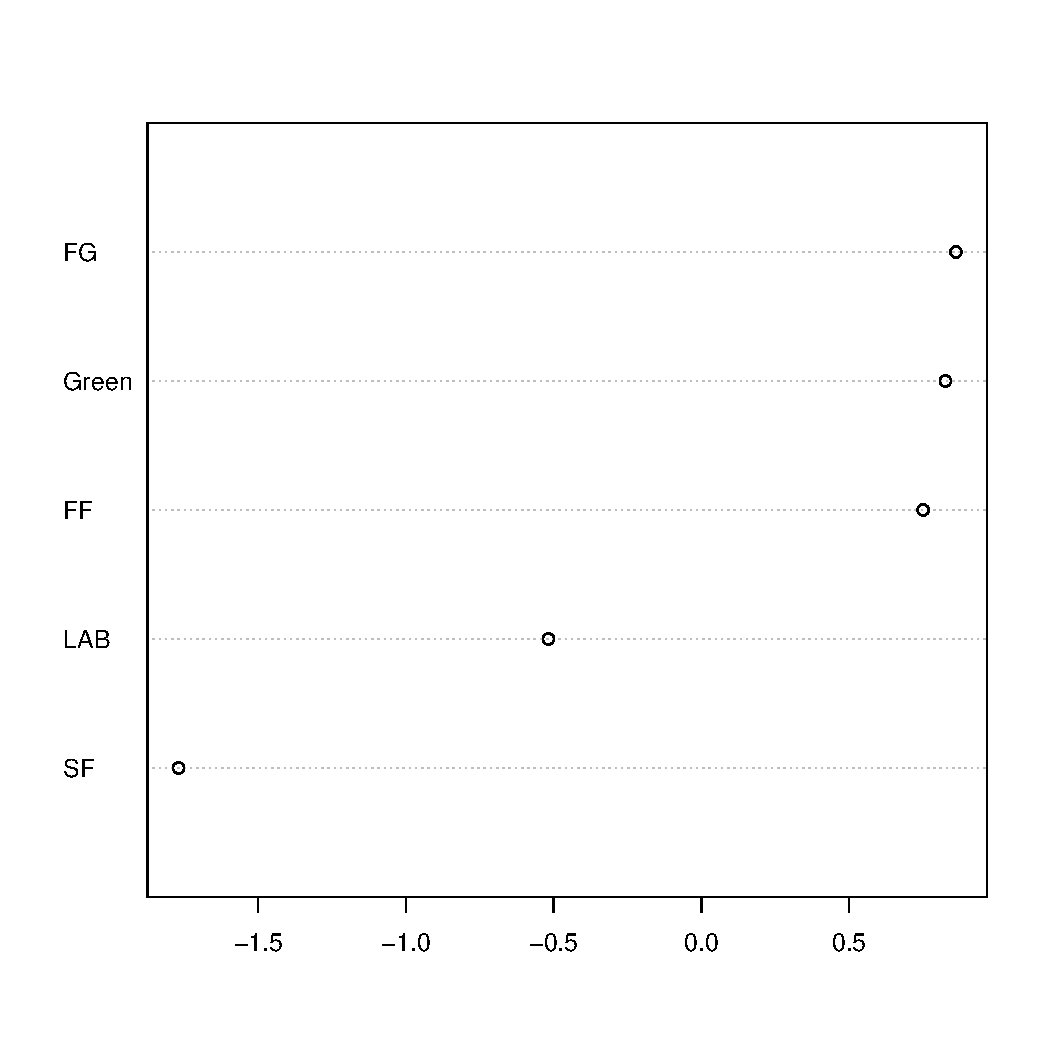
\includegraphics[width=\maxwidth]{figures/minimal-unnamed-chunk-9} 

}



\end{knitrout}

This plot indicates the position
of each of the documents. We can group documents by their attribute values when creating the word-frequency matrix: 

\begin{knitrout}\footnotesize
\definecolor{shadecolor}{rgb}{0.969, 0.969, 0.969}\color{fgcolor}\begin{kframe}
\begin{alltt}
\hlstd{partyMat} \hlkwb{<-} \hlkwd{dfm}\hlstd{(ieBudgets2010,} \hlkwc{group}\hlstd{=}\hlstr{"party"}\hlstd{)}
\end{alltt}
\begin{verbatim}
## Creating dfm: ... aggregating by group: party...complete ... done.
\end{verbatim}
\begin{alltt}
\hlstd{partyMat[,}\hlnum{1}\hlopt{:}\hlnum{5}\hlstd{]}
\end{alltt}
\begin{verbatim}
##        words
## docs      a abandoned abandoning abetted ability
##   FF     78         0          0       0       1
##   FG    162         0          0       0       1
##   Green 326         2          1       1       5
##   LAB   288         0          0       0       3
##   SF    159         0          0       0       1
\end{verbatim}
\end{kframe}
\end{knitrout}

which allows us to scale according to a particular party or year, for example:

\begin{knitrout}\footnotesize
\definecolor{shadecolor}{rgb}{0.969, 0.969, 0.969}\color{fgcolor}\begin{kframe}
\begin{alltt}
\hlstd{partyModel} \hlkwb{<-} \hlkwd{ca}\hlstd{(}\hlkwd{t}\hlstd{(partyMat),}\hlkwc{nd}\hlstd{=}\hlnum{1}\hlstd{)}
\hlkwd{dotchart}\hlstd{(partyModel}\hlopt{$}\hlstd{colcoord[}\hlkwd{order}\hlstd{(partyModel}\hlopt{$}\hlstd{colcoord[,}\hlnum{1}\hlstd{]),}\hlnum{1}\hlstd{],} \hlkwc{labels} \hlstd{= partyModel}\hlopt{$}\hlstd{colnames[}\hlkwd{order}\hlstd{(partyModel}\hlopt{$}\hlstd{colcoord[,}\hlnum{1}\hlstd{])])}
\end{alltt}
\end{kframe}

{\centering 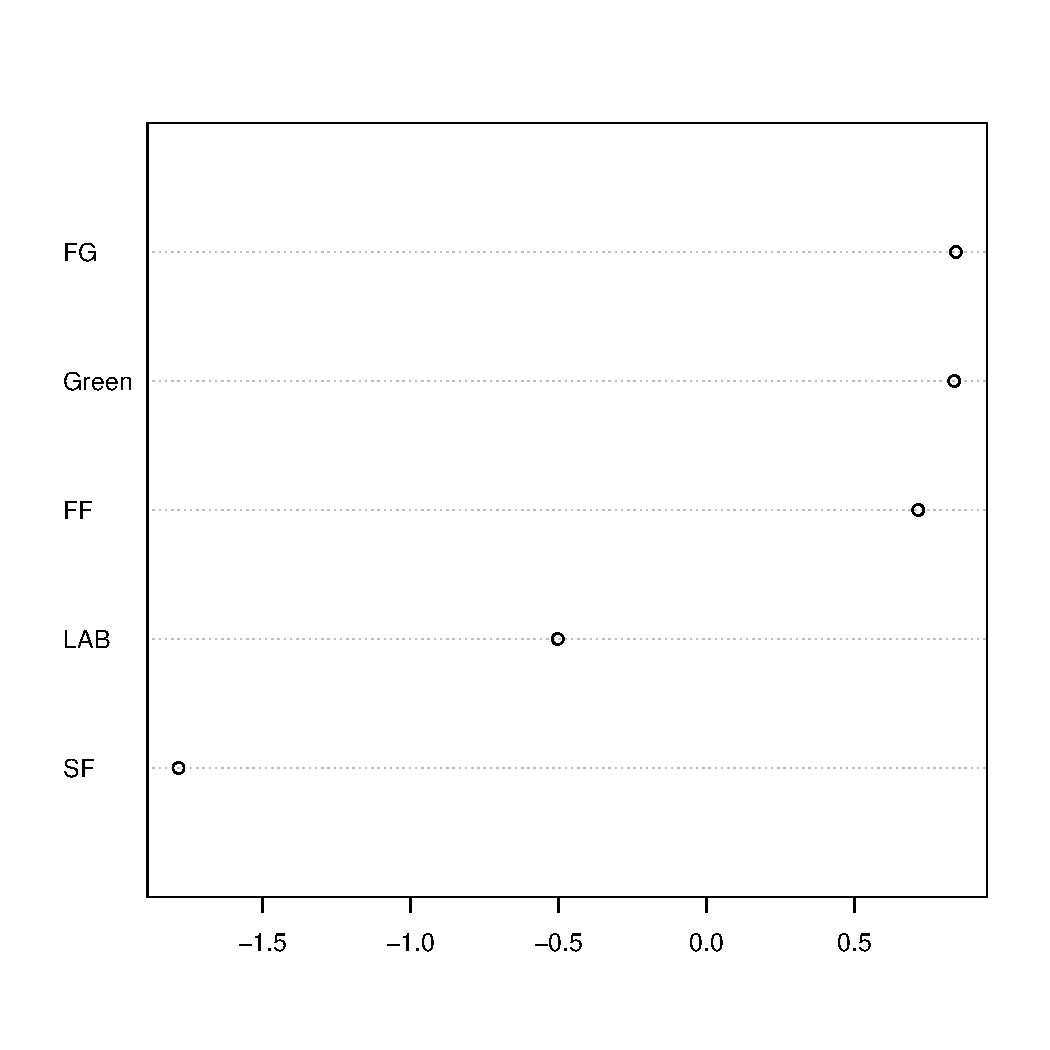
\includegraphics[width=\maxwidth]{figures/minimal-unnamed-chunk-11} 

}



\end{knitrout}

